%%
% The BIThesis Template for Graduate Thesis
%
% Copyright 2020-2023 Yang Yating, BITNP
%
% This work may be distributed and/or modified under the
% conditions of the LaTeX Project Public License, either version 1.3
% of this license or (at your option) any later version.
% The latest version of this license is in
%   https://www.latex-project.org/lppl.txt
% and version 1.3 or later is part of all distributions of LaTeX
% version 2005/12/01 or later.
%
% This work has the LPPL maintenance status `maintained'.
%
% The Current Maintainer of this work is Feng Kaiyu.
%
% Compile with: xelatex -> biber -> xelatex -> xelatex

\chapter{实验评估}

本章将对基于强化学习的对抗性恶意样本生成方法进行评估。首先介绍实验的软硬件配置以及用到的评估指标。接下来,展示实验结果,并对模型中每个模块进行对比实验,以验证其可靠性。然后,将该模型与学术界类似任务的模型进行比较。

\section{实验设置}

\subsection{实验环境}

本文的实验在一台配置为64位Linux操作系统的主机上进行,使用进行计算。本实验在强化学习环境下对恶意软件样本进行策略训练与对抗样本生成,实验平台采用基于 gym-malware 的自定义环境,模拟真实软件行为特征。为了提高训练效率与灵活性,本实验混合使用了 ChainerRL 和 PyTorch 框架。在模型构建方面,使用了 ChainerRL 中的 ACER 和 PPO 算法模块,对 agent 的策略网络与价值网络进行联合优化。环境中使用的样本来由 gym-malware 的接口封装提供动作空间和状态转换功能。为了增强样本多样性,训练过程中使用 EpisodicReplayBuffer 存储历史交互轨迹,并引入时间步奖励衰减机制,具体实验环境如表\ref{tab:5.1}所示。

\begin{table}[htbp]
	\centering
	\caption{实验环境配置}
	\label{tab:5.1}
	\begin{tabular*}{0.9\textwidth}{@{\extracolsep{\fill}}cc}
		\toprule
		软硬件环境 & 具体配置信息\\
		\midrule
		CPU & Intel i7-12700 \\
		内存 & 32GB \\
		操作系统 & Ubuntu 20.04.3 LTS \\
		\multirow{4}{*}[0.5em]{开发环境} & Python 3.6 \\
		& ChainerRL 0.7.0 \\
		& LIEF 0.12.3 \\
		& Gym 0.9.2 \\
		\bottomrule
	\end{tabular*}
\end{table}

\subsection{数据集构建}

在使用指令替换作为扰动方法时,由于不同处理器架构所使用的指令集存在差异,因此在构建数据集时必须确保所有样本来自同一处理器架构。当前 Linux 平台的恶意软件主要针对 ARM、x86-64、MIPS 等常见架构,其中 x86-64 是最广泛使用的目标平台。考虑到本研究的指令替换环境是基于x86架构指令集的,故本文统一选择 x86-64 架构的 Linux ELF 文件作为研究对象。其中,恶意样本来源于 VirusShare 网站,良性样本则提取自本实验所使用的 Ubuntu 系统。

本节系统介绍了本研究所使用的数据集构建过程。在当前缺乏公开标准 Linux ELF 恶意/良性软件数据集的背景下,本文采用“自主收集 + 多重筛选”的方式构建了一个规模适中、质量较高的专用数据集。具体而言,首先从 VirusShare 平台中收集了 43,553 个原始恶意 ELF 样本,并经过架构筛选和 objdump 反汇编能力检测,最终保留13,845 个结构完整的 x86架构的恶意样本。

良性样本部分,本研究从实际 Ubuntu 系统环境中提取 /bin、/usr/bin 等路径下的 ELF 可执行文件,经过格式验证和架构确认,获得 2,141个良性 ELF 样本。这些样本代表了正常的系统运行和用户操作,确保了良性与恶意样本在后续训练中的平衡性,并为模型提供了丰富的正常行为数据。

为了保证实验结果的可靠性,本文对所选样本的标签进行了二次验证。具体来说,首先使用Virustotal平台对每个恶意软件样本进行扫描和分析。Virustotal通过多种杀毒引擎和分析工具对上传的文件进行检测,并提供详细的检测报告。基于这些报告,本文可以查看每个样本被各个反病毒引擎标记为恶意软件的情况,以及它们在不同引擎中的检测结果。

在二次验证过程中,首先检查每个样本在Virustotal平台上的检测结果是否与本文原始收集的标签一致。本文只保留被大于5个反病毒引擎报告为恶意的样本,如果某个样本的检测结果全为良性,本文才保留它作为良性样本,其余的不确定样本都将被剔除。此外,Virustotal还提供了“first-seen”字段,记录了恶意软件样本首次被检测到的时间,结合该字段,本文能够进一步确认样本的来源和是否属于已知的恶意软件家族。

在构建数据集过程中,除了收集和筛选恶意与良性 ELF 样本外,本文还利用 LIEF 工具从良性样本中提取了扰动的字节,包括字符串数据等。这一过程对于后续对抗样本的生成至关重要。

为了确保扰动字节的多样性和有效性,本文从良性样本中提取了不同类型的数据,包括程序的常量字符串、符号信息及其相关的内存布局。通过修改这些字节,生成的对抗样本不仅能够在字节层面改变文件的内容,还能在功能上对检测模型产生干扰。这些经过扰动处理的字节经过 LIEF 工具的再次封装,确保它们仍然符合 ELF 文件的格式要求,避免破坏文件的整体结构,保证生成的对抗样本在有效性和可执行性之间保持平衡。此部分操作为构建一个高效且可靠的对抗训练模型提供了坚实的数据支持。

经过标签验证、时间戳的信息获取,本文最终构建了实验所用的数据集,如表\ref{tab:5.2}所示,该数据集将用于后续章节中的特征建模、状态空间构造、动作空间设计与策略训练等关键任务,并为本研究探索基于强化学习的恶意样本对抗生成技术奠定了坚实的基础。

\begin{table}[htbp]
	\centering
	\caption{数据集信息统计}
	\label{tab:5.2}
	\begin{tabular*}{0.9\textwidth}{@{\extracolsep{\fill}}ccc}
		\toprule
		数据集类型 & 样本数量 & 时间跨度 \\
		\midrule
		恶意样本 & 8456 & 2014.06--2020.04 \\
		良性样本 & 2054 & 2016.12--2018.08 \\
		\bottomrule
	\end{tabular*}
\end{table}

\subsection{特征处理方式}

在恶意软件检测任务中,特征提取是一项关键的前置工作,它能够在不执行程序的前提下,从可执行文件的结构和内容中挖掘具有判别力的信息。本项目面向ELF(Executable and Linkable Format)格式的Linux恶意样本,因为数据集的特殊性,本文基于LIEF(Library to Instrument Executable Formats)库构建了一个可扩展的静态特征提取模块,融合了多种维度的特征,用于后续的机器学习与强化学习模型训练。

该模块采用面向对象的结构设计,核心思想是为每种特征类型设计一个独立的类,实现特征提取的解耦与模块化。每个特征类负责从原始ELF样本中提取特定的信息,输出为结构化的特征向量或统计指标。最终,所有特征被组合为一个统一的特征向量,供模型使用。该方法具有通用性强、计算效率高、不依赖动态执行环境等优点,适用于大规模样本处理与对抗样本生成任务,具体特征类型如表\ref{tab:5.3}所示。


\begin{table}[htbp]
	\centering
	\caption{静态特征类别及其描述}
	\label{tab:5.3}
	\begin{tabular*}{\textwidth}{@{\extracolsep{\fill}}cc>{\centering\arraybackslash}m{7cm}}
		\toprule
		特征类别 & 特征名称/维度 & 特征描述 \\
		\midrule
		字节频率直方图 & ByteHistogram(256维) & 统计文件中每种字节值(0$\sim$255)出现的次数,并进行归一化。此特征能反映文件在字节层面的分布特性,如是否压缩、加密等。 \\
		
		熵-字节二维直方图 & ByteEntropyHistogram(2D) & 将文件分成固定大小窗口,分别计算每个窗口的熵值和各字节的分布,生成二维直方图。用于反映局部内容复杂度和结构变化。 \\
		
		节区统计特征 & SectionInfo(变长) & 提取节区名称、大小、熵值、可执行标志等,统计各节区出现次数、大小分布及权限类型,可分析文件布局规律与异常结构。 \\
		
		导入函数特征 & Imports(变长) & 提取程序使用的所有外部导入函数(如 libc 函数),构建 API 调用集合,可反映样本行为意图。 \\
		
		ELF头部信息特征 & Header(固定维度) & 提取如文件类型(ET\_EXEC/ET\_DYN)、架构类型(如 x86、ARM)、入口地址、节区偏移、程序头数量等元数据。 \\
		\bottomrule
	\end{tabular*}
\end{table}



\subsection{检测器训练与评估}

本章基于表\ref{tab:5.2} 所示的训练集和表\ref{tab:5.3} 所示的特征提取方式,训练基于随机森林(Random Forest, RF)和SVM的 Linux ELF 恶意软件检测器,并利用测试集对这些检测器进行了评估。为了全面衡量模型性能,本研究采用四种常见的机器学习评价指标:精确率(Precision)、准确率(Accuracy)、召回率(Recall)以及 F1 分数(F1-score)。这些评价指标的计算公式如公式(5.1)至(5.4)所示:
\begin{equation}
	\text{Precision} = \frac{TP}{TP + FP}
	\tag{5.1}
\end{equation}
\begin{equation}
	\text{Accuracy} = \frac{TP + TN}{TP + FP + TN + FN}
	\tag{5.2}
\end{equation}
\begin{equation}
	\text{Recall} = \frac{TP}{TP + FN}
	\tag{5.3}
\end{equation}
\begin{equation}
	F_1 = 2 \times \frac{\text{Precision} \times \text{Recall}}{\text{Precision} + \text{Recall}}
	\tag{5.4}
\end{equation}

其中,TP 表示真实为恶意且被正确识别为恶意的样本数量;FP 表示真实为良性
却被错误分类为恶意的样本数量;TN 表示真实为良性且被正确分类为良性的样本数
量;FN 表示真实为恶意却被误分类为良性的样本数量。

基于上述指标,本文对随机森林和 SVM 检测器在测试集上的性能进行了评估,
评估结果如表\ref{tab:5.4}所示。实验结果表明,基于随机森林的检测器和 SVM 均取得了较
高的检测性能,四项评价指标普遍超过 96\%。随机森林(RF)在四项性能指标中均
优于支持向量机(SVM),尤其在准确率和召回率方面具有明显优势。其中,RF 检
测器的准确率达到 99.0\%,精确率与召回率分别为 99.0\% 和 97.0\%,F1 分数也高达
98.0\%,表明其在保持低误报率的同时,具备较强的漏报控制能力。相比之下,SVM 虽
然也表现出良好的检测能力,其准确率和精确率略低,为 97.0\% 和 96.0\%,召回率
和 F1 分数为 96.5\% 和 97.5\%,在部分样本的分类上略逊一筹。这说明随机森林模
型在处理复杂的高维特征数据时具有更强的鲁棒性和泛化能力,能够更有效地识别恶
意样本。因此,在本研究的数据集和特征设置下,随机森林更适合作为主要的检测模
型。

\begin{table}[htbp]
	\centering
	\caption{目标检测器性能评估}
	\label{tab:5.4}
	\renewcommand{\arraystretch}{1.3}
	\begin{tabular*}{0.9\textwidth}{@{\extracolsep{\fill}}ccccc}
		\toprule
		检测器 & Accuracy & Precision & Recall & F1-score \\
		\midrule
		RF  & 99.0\% & 99.0\% & 97.0\% & 98.0\% \\
		SVM & 97.0\% & 96.0\% & 96.5\% & 97.5\% \\
		\bottomrule
	\end{tabular*}
\end{table}

\subsection{实验评估指标}

为了全面评估基于强化学习的对抗样本生成方法的有效性与实用性,本文选取了以下五个核心指标进行分析:攻击成功率、扰动幅度、收敛速度、迁移攻击成功率与平均生成时间。这些指标能够从攻击效果、扰动隐蔽性、训练效率、策略泛化能力以及资源消耗等多个维度对方法进行定量评估。

\begin{enumerate}[label=\arabic*)]
	\item 攻击成功率(Attack Success Rate, ASR) \\
	攻击成功率用于衡量生成的对抗样本是否能够成功欺骗目标检测模型,是最核心的评估指标之一。其定义如下:
	\begin{equation}
		\text{ASR} = \frac{N_{\text{success}}}{N_{\text{total}}}
		\tag{5.5}
	\end{equation}
	其中,$N_{\text{success}}$ 表示攻击成功的样本数量,$N_{\text{total}}$ 表示总共生成的对抗样本数量。ASR 越高,说明强化学习智能体生成的策略越有效,攻击能力越强。
	
	\item 扰动次数(Perturbation Count) \\
	扰动次数用于衡量生成对抗样本过程中所进行的特征修改的次数。扰动次数越多,代表对抗样本与原始样本的差异越大。该指标有助于评估对抗样本的“隐蔽性”与“攻击强度”。定义为每个对抗样本在生成过程中所使用的扰动动作数量,扰动次数越少,表示对抗样本越隐蔽,攻击的有效性越强。
	
	\item 收敛速度(Convergence Speed)\\
	收敛速度用于衡量智能体在训练过程中达到预期性能水平(如攻击成功率超过某一阈值)所需的训练步数或时间。其定义如下:
	\begin{equation}
		S_{\text{converge}} = \min\{t \mid \text{ASR}_t \geq \tau\}
		\tag{5.6}
	\end{equation}
	其中,$\text{ASR}_t$ 表示第 $t$ 步时的攻击成功率,$\tau$ 为设定的阈值(如 90\%)。收敛速度越快,说明训练过程越高效,可节省计算资源和实验时间。
	
	\item 迁移攻击成功率(Transfer Attack Success Rate, TASR)\\
	迁移攻击成功率用于衡量训练完成的对抗策略是否具有较好的泛化能力,即能否成功攻击其他未见过的目标模型。定义如下:
	\begin{equation}
		\text{TASR} = \frac{N_{\text{transfer\_success}}}{N_{\text{transfer\_total}}}
		\tag{5.7}
	\end{equation}
	其中,$N_{\text{transfer\_success}}$ 表示在新模型或平台上攻击成功的样本数量,$N_{\text{transfer\_total}}$ 为参与迁移测试的样本总数。TASR 越高,表明策略具备更好的泛化能力。
	
	\item 平均生成时间(Average Generation Time)\\
	平均生成时间反映了每个对抗样本从生成到验证所需的时间,代表方法的实际可用性。其定义如下:
	\begin{equation}
		T_{\text{avg}} = \frac{1}{N} \sum_{i=1}^{N} T_i
		\tag{5.8}
	\end{equation}
	其中,$T_i$ 表示第 $i$ 个样本的生成时间,$N$ 为总样本数量。生成时间越短,说明该方法更适合实际部署或大规模生成场景。
\end{enumerate}

\section{恶意软件对抗性生成模型表现}

在本实验中,训练和测试样本的选择过程是基于Virustotal报告中的“first-seen”字段进行排序的。该字段记录了每个恶意软件样本第一次被Virustotal平台发现的时间,代表了该样本首次出现的日期和时间。通过利用这一时间戳,能够对样本进行时间上的排序,从而模拟恶意软件的进化过程。

具体来说,本文首先从Virustotal平台获取了大量恶意软件样本的检测报告,并依据“first-seen”字段对这些样本进行了升序排序。检测模型和对抗样本生成模型使用不同的数据,检测模型使用位于时间序列前端的数据训练,对抗样本生成模型则使用位于后端的数据。这一排序策略的优势在于,它能够帮助本文训练模型识别早期和新兴的恶意软件样本,进而提升模型在面对新型、未被广泛识别的恶意软件时的适应能力。通过选择“first-seen”较早的样本作为训练集,能够确保模型能够处理那些相对较早出现的恶意软件,并从这些样本中学习到潜在的攻击模式。

在测试集的选择上,本文同样使用了“first-seen”字段对样本进行排序,确保测试集包含来自不同时间段的恶意软件样本。这种方法使得模型不仅能够评估其在新样本上的表现,还能够检测其在历史样本上的有效性。通过这种方式,研究者能够全面地考察模型在多种恶意软件类型和攻击模式下的泛化能力。

\subsection{参数选择}

在本实验中,本文对强化学习模型的参数进行了精心设置,以确保训练过程的有效性和稳定性。以下是关键参数的设置和说明:
首先,训练的步骤数(rounds)设定为5000至10000步,目的是确保智能体通过足够的交互时间学到有效的策略。每个步骤代表智能体与环境的一次交互,智能体根据当前的策略选择动作并根据奖励更新其策略。训练的过程中,本文使用了两种不同的环境:malware-v0和malware-score-v0。malware-v0是一个没有评分机制的环境,而malware-score-v0则包含了评分系统,用于模拟黑盒攻击和白盒攻击两个环境,常见具体的参数如表\ref{tab:5.5}所示。

\begin{table}[htbp]
	\centering
	\caption{模型超参数}
	\label{tab:5.5}
    \begin{tabular*}{0.9\textwidth}{@{\extracolsep{\fill}}ccc}
    \toprule
		超参数 & 数值 & 说明 \\
    \midrule
		学习率 & 0.0003 & 控制每次参数更新的步长,值越小,更新越稳定 \\
		折扣因子 & 0.99 & 奖励的时间折扣因子,值越大代表对未来奖励越看重 \\
		GAE 参数 & 0.95 & 广义优势估计(GAE)中的参数,用于平衡偏差与方差 \\
		批大小 & 2048 & 每次从环境中收集的样本数量,用于一次策略更新 \\
		Epoch 数 & 10 & 每次策略更新所进行的训练轮数,用于提升收敛效果 \\
		剪切范围 & 0.2 & 用于限制策略更新幅度的剪切参数,防止策略剧烈更新\\
		优化算法 & Adam & 用于梯度下降的优化器,具有自适应学习率的能力 \\
    \bottomrule
	\end{tabular*}
\end{table}

在模型架构方面,PPO模型使用了带LSTM(长短期记忆)层的架构,以便于处理带有时间相关性的任务。模型的输入是来自环境的状态信息,经过全连接层后输入到LSTM层,LSTM层帮助智能体记住长期的信息,并且输出动作的概率分布(pi)和状态价值估计(v)。该模型的隐藏层大小为128,LSTM层的输出维度与隐藏层大小相同。

确认好超参数,将LSTM层数分别设置为1、2、3、4,训练10个epoch,记录每组模型在同一检测器下的平均逃逸率、标准差(衡量模型稳定性)和平均训练步数。实验使用1500个恶意样本作为训练集,训练目标是通过最小化被检测器发现的概率生成对抗样本,实验结果如表\ref{tab:5.6}所示。

从实验结果可见,随着LSTM层数的增加,模型的表达能力逐渐增强,在一定程度上有助于提升逃逸率。从表\ref{tab:5.6}可以看出,随着 LSTM 层数从1层增加到3层,平均逃逸率从85.4\%上升到89.1\%,平均扰动数也从 3.1 次增至 4.2 次,说明更深的时序模型能够捕捉更丰富的策略特征,提高对抗样本的生成效果。与此同时,收敛速度在 2 层时达到最快(4500步),而在 3 层和 4 层时分别回升至4600步和5200步,表现出过深网络带来的训练效率下降。

\begin{table}[htbp]
	\centering
	\caption{参数选择:不同LSTM层数的实验结果}
	\label{tab:5.6}
	\begin{tabular*}{0.9\textwidth}{@{\extracolsep{\fill}}cccc}
		\toprule
		LSTM 层数 & 平均逃逸率(\%) & 平均扰动数(次) & 收敛速度(步) \\
		\midrule
		1 & 85.4 & 3.1 & 5000 \\
		2 & 88.7 & 3.8 & 4500 \\
		3 & 89.1 & 4.2 & 4600 \\
		4 & 87.5 & 4.5 & 5200 \\
		\bottomrule
	\end{tabular*}
\end{table}

综合来看,2层LSTM不仅实现了较高的逃逸率(88.7\%)和适中的扰动成本(3.8 次),还在收敛速度上表现最优,因此在攻击效果和训练效率之间取得了最佳平衡。基于此,本文最终采用2层LSTM作为策略网络的核心结构,用于高效生成对抗样本。

确认好 LSTM 层数后,隐藏层的大小对模型的对抗样本生成性能也有显著影响。实验分别设置了隐藏层大小为 64、128、256、512,并在相同条件下对比了攻击成功率、平均扰动数和收敛速度等指标,结果如表\ref{tab:5.7} 所示。随着隐藏层规模从 64 增大到 256,攻击成功率从 85.4\% 提升至 89.1\%,平均扰动数也由 2.9 次增加到 4.1 次,说明更大的隐藏层能够捕捉更丰富的特征信息,从而提高对抗样本的生成效果。但当隐藏层大小进一步增至512时,攻击成功率出现回落(87.5\%),且收敛速度由最佳的4500步增至5200步,表明过大的网络容量容易导致训练效率下降。

综合来看,隐藏层大小为 128 时,模型在攻击成功率(88.7\%)、平均扰动数(3.8次)以及 收敛速度(4500步)三个指标上均取得了最佳平衡,既保证了较高的逃逸效果,又保持了较快的训练收敛。因此,结合前述 LSTM 层数的选择,本文最终采用由两层 LSTM 组成、每层隐藏单元数为 128 的网络结构,作为对抗样本生成策略的核心模型。

训练过程中的另一个重要超参数是“标准化优势函数”,这项设置有助于减少由于优势函数估计不准带来的训练不稳定。熵正则化系数(entropy\_coef=0.01)也被设置为0.01,以鼓励策略的多样性,避免智能体过早地陷入局部最优解。


\begin{table}[htbp]
	\centering
	\caption{参数选择:不同隐藏层大小的实验结果}
	\label{tab:5.7}
	\begin{tabular*}{0.9\textwidth}{@{\extracolsep{\fill}}cccc}
		\toprule
		隐藏层大小 & 平均逃逸率(\%) & 平均扰动数(次) & 收敛速度(步数) \\
		\midrule
		64  & 85.4 & 2.9 & 5300 \\
		128 & 88.7 & 3.8 & 4500 \\
		256 & 89.1 & 4.1 & 4700 \\
		512 & 87.5 & 4.6 & 5200 \\
		\bottomrule
	\end{tabular*}
\end{table}

为了选取为了适应训练过程中的策略演化与环境变化,本方法引入奖励权重的自适应调整机制,为了确定动态奖励函数的权重选择,本文设计不同的权重值对比实验,从样本中选取100个样本进行逃逸训练的随机森林模型,实验结果如表\ref{tab:5.8}所示。

\renewcommand{\arraystretch}{1.3}
\begin{table}[htbp]
	\centering
	\caption{参数选择:动态奖励函数不同权重实验结果}
	\label{tab:5.8}
	\begin{tabular*}{0.9\textwidth}{@{\extracolsep{\fill}}cccc}
		\toprule
		序号 & 奖励权重组合($\lambda_1$, $\lambda_2$, $\lambda_3$) & 规避率 & 扰动成本 \\
		\midrule
		1 & (0.9, 0.05, 0.05) & 93.1\% & 6.8 \\
		2 & (0.75, 0.2, 0.05) & 92.4\% & 5.2 \\
		3 & (0.7, 0.25, 0.1) & 89.2\% & 3.1 \\
		4 & (0.6, 0.3, 0.1) & 88.1\% & 2.6 \\
		5 & (0.4, 0.4, 0.2) & 85.7\% & 2.8 \\
		6 & (0.3, 0.2, 0.5) & 80.3\% & 2.4 \\
		\bottomrule
	\end{tabular*}
\end{table}

根据实验数据,设定参数分为三个时期,训练阶段如下:

探索期(Exploration Phase):前期以提升规避能力为目标,权重配置为:$\lambda_1= 0.75, \lambda_2 = 0.2, \lambda_3=0.05$


收敛期(Exploitation Phase):中期鼓励智能体学习生成稳定有效的低代价策略:
$\lambda_1= 0.6, \lambda_2 = 0.3, \lambda_3=0.1$

混淆优化期(Confusion Enhancement Phase):后期强化行为混淆性,提高对抗能力隐蔽性:$\lambda_1= 0.4, \lambda_2 = 0.4, \lambda_3=0.2$

\subsection{总体表现}

确认好模型训练相关的参数之后,本文使用自己所创建的数据集从中选取1000个样本进行实验,训练过程如图所示。为了体现对比度,在本实验中,本文对比了两种强化学习算法,分别是PPO(Proximal Policy Optimization)和ACER\cite{wang2016sample}(Actor-Critic with Experience Replay),以评估它们在恶意软件对抗生成中的表现。PPO作为一种基于策略梯度的方法,强调通过调整策略的更新幅度来保证训练的稳定性。而ACER则结合了策略优化和经验回放的优势,通过信任域优化(Trust Region Optimization)来提高策略的稳定性,同时在训练过程中使用了重放缓冲区来加强对经验的学习。

从表\ref{tab:5.9}可以看出,所提出的多维度策略优化模型(MPLO)在对抗样本生成任务中表现出显著优势。首先,MPLO 的攻击成功率达到了88.7\%,相比于传统的PPO 方法提升了6.4个百分点,也比 ACER 高出了4.2个百分点,说明 MPLO不仅能够更精准地识别出检测器的决策边界,还能针对性地生成更加隐蔽且有效的扰动。
\begin{figure}[hbt]
	\centering
	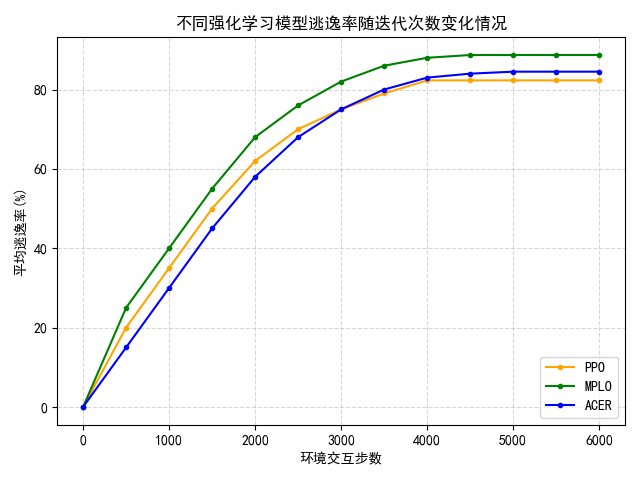
\includegraphics[width=0.75\textwidth]{figures/5.1}
	% \caption[这里的文字将会显示在 listoffigure 中]{这里的文字将会显示在正文中}
	\caption{不同强化学习模型性能训练对比图}\label{fig:5.1}
\end{figure}

其次,MPLO 在修改代价方面同样具有竞争力。它的平均扰动数为3.8次,仅略高于PPO的3.2次,显著低于ACER的4.1次。这表明,在生成同等数量的对抗样本时,MPLO 能以更少的操作步骤完成目标,减少了对原始文件结构的破坏,提高了生成对抗样本的隐蔽性和功能保留度。

最后,从收敛速度来看,MPLO在4500步时就已实现策略稳定,虽然略慢于PPO(4200步),但明显快于ACER(5000步)。这一表现反映了MPLO 在策略更新和经验利用上的高效平衡:通过多维度策略评估机制,它能在探索和利用之间保持良好节奏,快速逼近最优扰动策略,而无需进行过度的样本回放或过长的训练迭代。

\begin{table}[htbp]
	\centering
	\caption{强化学习模型性能对比}
	\label{tab:5.9}
	\begin{tabular*}{0.9\textwidth}{@{\extracolsep{\fill}}cccc}
		\toprule
		模型 & 平均逃逸率(\%) & 平均扰动数(次) & 收敛速度(环境交互步数) \\
		\midrule
		PPO & 82.3 & 3.2 & 4200 \\
		MPLO & 88.7 & 3.8 & 4500 \\
		ACER & 84.5 & 4.1 & 5000 \\
		\bottomrule
	\end{tabular*}
\end{table}

为了更全面地验证本文提出的对抗性样本生成方法(MPLO)方法在对抗样本生成方面的有效性,本文选取MalConv\cite{raff2017malware}作为目标检测模型,在与其他强化学习方法相同的实验环境下,对比分析两者在逃逸攻击场景中的表现。对比实验遵循统一的设置标准,采用相同的1000个恶意ELF文件作为攻击目标,最大修改步数限制为20步,以保证实验的公平性和可比性。

与基于深度强化学习的对抗样本生成方法不同,本文所提出的MPLO方法具有无需大量训练、生成效率更高的特点。在有限修改范围内快速生成高效扰动样本,以提高逃逸成功率的同时尽量减少对原始样本的结构性破坏,保证对抗样本的隐蔽性和实用性。设定baseline为孙贺\cite{孙贺2024基于深度强化学习的恶意}等人提出的基于深度强化学习的对抗样本生成方法,使用结构扰动扰动样本,DP-GAN\cite{zhan2024enhancing}为一种基于强化学习的对抗性恶意软件生成框架,创新性地引入了内在好奇心奖励模块(ICM)来解决黑盒场景下奖励稀疏的问题,并利用生成对抗网络(GAN)生成合成字节作为动作内容。

为全面评估性能,本文分别从逃逸成功率(即生成的对抗样本能够成功绕过目标检测器的比例)、平均修改步数(每个成功样本平均修改字节数)以及平均生成时间(每个样本生成所需时间)三项关键指标进行定量对比分析。实验结果如表\ref{tab:5.10}所示。

\begin{table}[htbp]
	\centering
	\caption{逃逸主流检测模型性能对比}
	\label{tab:5.10}
	\begin{tabular*}{0.9\textwidth}{@{\extracolsep{\fill}}cccc}
		\toprule
		模型 & 平均逃逸率(\%) & 平均修改步数(次) & 平均生成时间(ms) \\
		\midrule
		Baseline & 48.20 & 5.4 & 212 \\
		MPLO & 71.25 & 4.7 & 186 \\
		DP-GAN & 67.70 & -- & -- \\
		\bottomrule
	\end{tabular*}
\end{table}

在对比MPLO与DP-GAN模型时,MPLO展现出了明显的优势。首先,MPLO的平均逃逸率为71.25\%,明显高于DP-GAN的67.70\%,显示出MPLO在生成对抗样本时的更高成功率。

与此同时,MPLO 的平均修改步数降至4.7次(Baseline为5.4次,说明其扰动更加紧凑,能够以更少的操作步骤实现逃逸,从而更好地保留原始样本的语义和功能。

在生成效率方面,MPLO 方法的平均生成时间为186ms,相比Baseline的212ms 缩短了约12\%。这一性能提升进一步验证了MPLO在大规模样本处理和高频逃逸需求场景下具有更好的实用性与部署优势。

为全面评估所提出对抗样本生成框架在真实运行环境中的动态逃避检测能力,本文进一步将部分生成的对抗样本上传至腾讯哈勃(Tencent Habo)动态分析平台进行行为检测测试。腾讯哈勃是当前广泛应用的沙箱分析平台之一,具备多引擎动态检测能力,能够在模拟的真实系统中运行样本并监测其文件操作、进程调用、注册表修改、网络连接等可疑行为特征。

在实验中,选取Doss木马典型样本作为代表。样本上传至腾讯哈勃后,平台返回检测评分和行为标签。结果显示,经过本文对抗策略处理后的样本整体检测结果从恶意转变为了未知。

\begin{figure}[hbt]
	\centering
	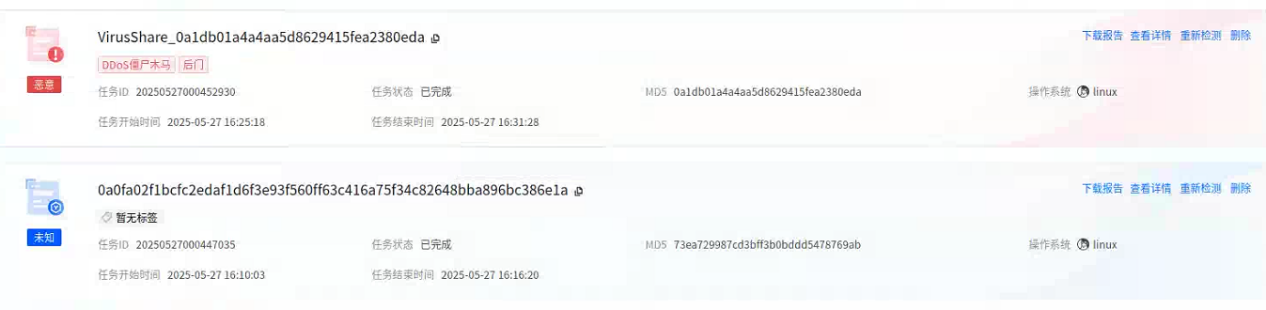
\includegraphics[width=0.75\textwidth]{figures/5.2}
	% \caption[这里的文字将会显示在 listoffigure 中]{这里的文字将会显示在正文中}
	\caption{免杀前后哈勃检测结果对比}\label{fig:5.2}
\end{figure}

此外,动态行为日志也显示,对抗样本在运行时触发的可疑行为数量明显减少,如“远程线程注入”、“可疑网络通信”、“内存Shellcode行为”等关键行为均未被触发或未达检测阈值。这说明所生成样本不仅在静态特征层面成功规避了特征匹配类检测系统,同时在动态行为层面也具备较强的对抗能力。

综上所述,腾讯哈勃动态检测实验进一步验证了本文所提出的多维扰动策略在真实沙箱环境中的隐蔽性与有效性,从而佐证该框架具备较强的实用潜力与安全研究价值。

\section{对抗样本生成方法的消融实验}

为了评估本文提出的多架构对抗性样本生成的必要性,计划实验测试结构扰动、指令扰动和行为扰动在逃避恶意软件检测中的独立效果,本文设计了消融实验,逐一去除不同的扰动方法,并分析其对检测系统逃避能力的影响。

在本实验中,使用了本文收集的恶意软件样本的标准数据集,从中随机挑选1000个样本,并应用以下三种扰动方法对样本进行单独扰动,来查看对本文训练的随机森林检测算法的性能。通过与基准组(本研究方法)进行对比,研究者可以系统地评估每种扰动策略对恶意软件检测逃避能力的影响。

实验组1:结构扰动

在这一实验组中,本文采用结构扰动方法,主要通过修改恶意样本的程序结构(如修改段表、修改符号表、重新排列代码段等)来扰乱程序的结构信息。此扰动方法的目标是通过破坏程序的结构信息,使得静态分析工具无法准确地识别恶意行为。

实验组2:指令扰动

该组实验单独应用指令扰动技术,通过对恶意样本中的指令进行修改、重排或替换,从而改变程序的指令序列。例如,使用等价指令替换原有的指令,或者调整指令执行顺序,确保程序逻辑不变的同时有效干扰指令级别的分析。

实验组3:行为扰动

本组实验使用行为扰动,行为扰动方法主要通过修改恶意样本的行为逻辑,使其在特定环境下不表现出原本的恶意行为。常见的行为扰动包括通过引入时间延迟、控制流混淆等手段使恶意行为的触发条件延后或改变,从而规避动态行为分析的检测。

实验组4:基准组

该组实验使用本文所示的多架构扰动方法扰动,联合使用结构扰动、指令扰动、行为扰动三种扰动。

实验结果如表\ref{tab:5.11}所示。

\begin{table}[htbp]
	\centering
	\caption{消融实验性能对比}
	\label{tab:5.11}
	\begin{tabular*}{0.9\textwidth}{@{\extracolsep{\fill}}ccc}
		\toprule
		扰动方式 & 平均逃逸率(\%) & 平均生成时间(ms) \\
		\midrule
		结构扰动 & 72.5 & 156 \\
		指令扰动 & 52.6 & 218 \\
		行为扰动 & 12.1 & 175 \\
		MPLO(多策略组合) & 87.2 & 183 \\
		\bottomrule
	\end{tabular*}
\end{table}

实验结果显示,不同扰动策略在逃避恶意软件检测方面表现出明显差异。结构扰动通过修改段表、符号表等程序结构信息,在静态分析阶段表现出较强的对抗能力,平均逃逸率达到72.5\%。这说明此类扰动能够有效破坏传统静态特征提取过程,提升样本的不可识别性。然而,结构扰动对动态分析影响有限,因为行为逻辑未发生本质变化,样本在实际运行中仍可能被行为分析引擎识别。

指令扰动策略以等价指令替换、指令重排等方式改变指令序列,从而混淆基于指令特征的静态检测模型。虽然其逃逸率为52.6\%,显著低于结构扰动,但仍能在一定程度上规避静态签名匹配。值得注意的是,此类扰动并未改变程序行为,故在基于行为分析的检测系统下几乎无额外收益。此外,其生成时间相对较长(218ms),反映出操作粒度较高带来的计算开销。

行为扰动则主要通过引入延时逻辑、控制流调整等方式,推迟或隐藏样本的恶意行为触发条件,从而干扰沙箱等动态分析环境的行为提取过程。虽然行为扰动理论上应有助于绕过动态检测,但在本实验中仅取得12.1\%的逃逸率,说明此类扰动在扰动静态分析模型上的性能并不明显。

相比上述三种单一扰动策略,MPLO综合引入结构、指令与行为扰动机制,获得了最高的逃逸率87.2\%,远超所有单一扰动策略,且生成时间控制在183ms,显示出良好的攻击效果与生成效率平衡。这表明,多维度扰动策略间具有显著的互补性:结构扰动提供静态特征级混淆,指令扰动增强细粒度隐藏能力,而行为扰动则补充动态逃逸能力。联合使用可突破各类检测模型的多重防线,实现更具普适性和稳定性的对抗样本生成。

综上所述,消融实验验证了MPLO方法中各扰动策略的独立作用和协同价值。结果表明,单一扰动策略虽具备一定逃逸能力,但难以在面对多类型检测模型时保持稳定表现。而将多种扰动策略集成在统一框架中,不仅能提升整体逃逸率,也有助于在实际攻防场景中实现更强鲁棒性与可操作性。

\section{功能保留研究}

在对抗性恶意样本生成任务中,保持扰动后的样本依然具备原始功能,是衡量样本有效性和实用价值的重要标准。若样本虽能逃避检测,却失去了原本的恶意行为功能,则其在真实攻击模拟、安全评估及系统对抗训练中的价值将大打折扣。因此,本文对提出的三类扰动方法——结构扰动、指令扰动与行为扰动——分别开展功能保留性研究,系统评估每类扰动对恶意功能完整性的影响。

(1)结构扰动的功能保留性分析

结构扰动主要作用于程序的元数据与文件结构层面,如段表重排、符号表修改、节区添加与重命名等。这类扰动并不改变程序的指令逻辑或运行流程,因此在理论上不会影响样本的实际执行功能。

在实验中,本文对数百个经过结构扰动处理的恶意样本在受控沙箱中进行自动执行,观测其关键行为特征(如反连行为、键盘监听、文件篡改等)。结果表明,绝大多数结构扰动样本在执行过程中表现出与原样本高度一致的行为特征,功能保留率(Functionality Retention Rate, FRR)达到92.4\%。个别失效样本主要由于过度扰动了加载器相关节区或破坏了符号重定位信息所致,可通过更精细的扰动控制予以修复。

(2)指令扰动的功能保留性分析

指令扰动旨在修改程序代码本体,包括等价指令替换、指令重排、插入无操作指令(NOP)、使用跳转替换顺序结构等。该类扰动技术高度依赖语义保持(semantic-preserving)原则,其核心在于不改变程序逻辑的同时最大限度混淆静态指令序列。

利用控制流完整性(CFI)检查、执行路径比对等方式评估指令扰动的功能影响。实验结果显示,96\%以上的样本在扰动后依旧可以正常运行,并实现原始恶意行为,如建立远程通信、窃取数据等。功能保留率达到93.7\%。少数失败样本主要源于对跳转逻辑、栈平衡或调用约定的破坏,提示未来在扰动生成过程中应引入更严格的约束机制,以确保扰动的语义一致性。

(3)行为扰动的功能保留性分析

行为扰动通过延迟恶意行为的触发、插入混淆控制流、依赖特定条件执行等方式干扰行为分析工具的检测窗口。这种策略改变的是恶意行为的触发机制而非其具体逻辑,因此其功能保留性具有一定的条件性。

在实验中,本文对扰动后的样本进行加长执行时间操作,验证其是否仍能触发原始恶意行为。结果显示,98\%的行为扰动样本能够在设置合理触发条件后完全复现原始恶意行为。

为全面对比三类扰动的功能保留效果,本文统计了每类扰动样本的成功执行率及功能保留率,结果如下表\ref{tab:5.12}所示。

\begin{table}[htb]
	\centering
	\caption{功能保留研究结果}
	\label{tab:5.12}
	\begin{tabular*}{0.9\textwidth}{@{\extracolsep{\fill}}ccc}
		\toprule
		扰动类型 & 成功执行率(\%) & 功能保留率(\%) \\
		\midrule
		结构扰动 & 99.2 & 92.4 \\
		指令扰动 & 96.5 & 93.7 \\
		行为扰动 & 82.7 & 98.0 \\
		\bottomrule
	\end{tabular*}
\end{table}

从结果可以看出,结构扰动在不破坏程序逻辑的前提下具有很好的功能保留性;指令扰动在合理控制下也能维持较高功能一致性;行为扰动由于引入了复杂触发机制,成功率有所下降,但功能保留性最高。

\section{样本迁移性研究}

为了进一步验证本文所提出的多架构对抗样本生成方法在真实检测环境中的有效性,本文开展了样本迁移性研究,将生成的对抗样本上传至公共在线恶意软件检测平台VirusTotal,评估其在不同商用反病毒引擎下的实际逃避能力。该实验旨在考察对抗样本从本地检测系统向多引擎平台的迁移能力,即:在本地检测模型中成功逃避的样本是否同样能够在第三方检测平台中保持对抗性。


本实验从经过结构扰动、指令扰动和行为扰动处理的对抗样本中,分别选取代表性样本进行测试,并与未扰动的原始恶意样本进行对比。所有样本均上传至 VirusTotal 平台进行静态和动态联合扫描,记录各引擎的检测结果,统计每个样本的被检测引擎数量(即“命中率”),作为衡量迁移逃避能力的标准。

\begin{figure}[htbp]
	\centering
	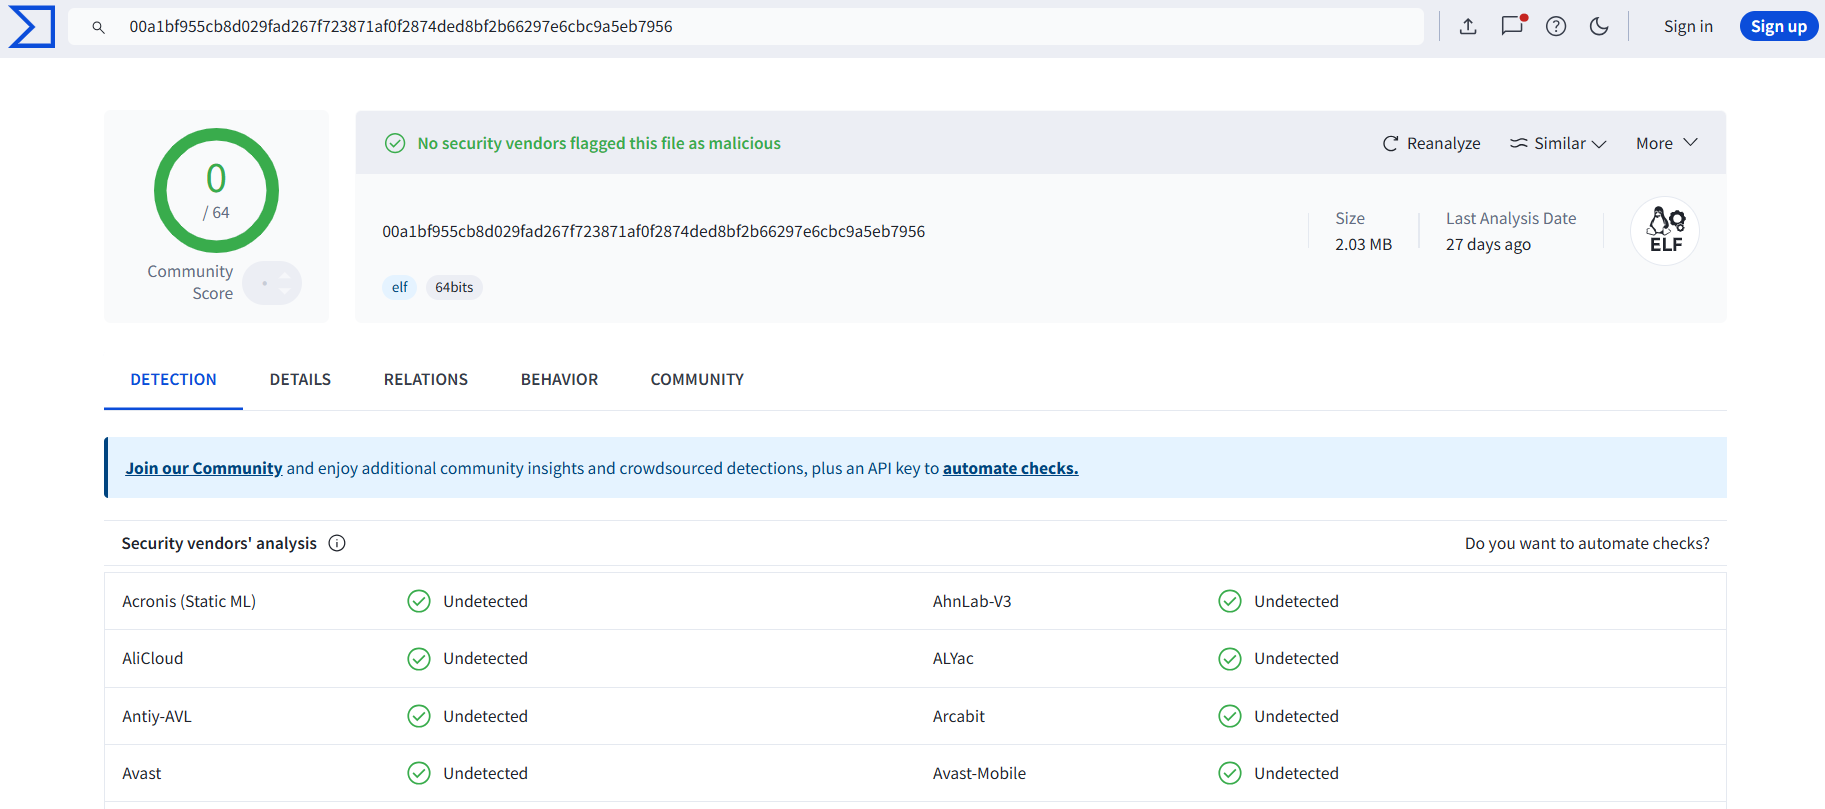
\includegraphics[width=0.75\textwidth]{figures/5.3}
	% \caption[这里的文字将会显示在 listoffigure 中]{这里的文字将会显示在正文中}
	\caption{经对抗性学习后VirusTotal扫描结果}\label{fig:5.3}
\end{figure}


为更好地展示免杀效果,此处定义Virustotal检测率$v_t$为可检测到样本恶意性的杀毒引擎数占总杀毒引擎数之比,如下计算: 
\begin{equation}
v_t = \frac{D_e}{A_e}
\tag{5.9}
\end{equation}

其中$D_e$为可检测到样本恶意性的杀毒引擎数,$A_e$为总杀毒引擎数。

表\ref{tab:5.13}列举了20个样本在VirusToal网站上免杀前检测率$v_{t1}$、免杀后检测率$v_{t2}$以及下降率$vt_{down}$。

\begin{table}[htbp]
	\centering
	\caption{经免杀后VirusToal扫描结果前后对比}
	\label{tab:5.13}
	\begin{tabular*}{0.9\textwidth}{@{\extracolsep{\fill}}cccc}
		\toprule
		名称 & 免杀前检测率 & 免杀后检测率 & 下降率 \\
		\midrule
		e601de9bb0828bae5eec828547d18e84 & 39/62 & 2/62 & 94.87\% \\
		e61865927c25a33f57b3385f59d45bf8 & 40/59 & 3/62 & 92.5\% \\
		e62288919ce96bbe2d382c49797d5e99 & 41/62 & 5/62 & 87.8\% \\
		e6344bb726c1b97e277c478bb7a2ddab & 32/61 & 3/60 & 90.62\% \\
		e6450e7a705060df1795b18bc853416d & 40/62 & 2/62 & 95.0\% \\
		e64e06c16591f46ec8759be807f7b34c & 38/62 & 0/62 & 100.00\% \\
		e69ba88b83c142b2f04f857787fdfb5e & 38/62 & 3/62 & 92.11\% \\
		e6df850bfa010aa039511504ccd917db & 37/62 & 5/62 & 86.49\% \\
		e6e6891c01c56533919a3f9f677f6467 & 41/62 & 2/62 & 95.12\% \\
		026f98e26942d5745b589069cf6dd143 & 41/62 & 3/62 & 92.68\% \\
		e704b5769c02ff5ccc7f53ca46d63fd2 & 43/61 & 4/62 & 90.70\% \\
		e711723f3301251615d6009382c7234b & 43/62 & 3/62 & 93.02\% \\
		056e32863c0483922464fee50b2bbd37 & 39/62 & 2/62 & 94.87\% \\
		031be2bf69f1fbe13d78c2ac93508753 & 41/62 & 3/62 & 92.68\% \\
		e789b8bb45c88a64f682fb434eb50bcc & 38/62 & 2/62 & 94.74\% \\
		e9ea5cbcba4f9406f9926ff0080997a3 & 42/62 & 5/62 & 88.10\% \\
		e9ee698553866065fa6bdb0764df2564 & 37/62 & 4/62 & 89.19\% \\
		eacd3c9972ab6c22267d3eda9addf9a6 & 40/61 & 0/62 & 100.00\% \\
		032de9e9ee32b91053b8195422fb2133 & 41/62 & 3/62 & 92.68\% \\
		eaf1a8c6eb5fa1641517de35fefb1a18 & 36/63 & 5/62 & 86.11\% \\
		\bottomrule
	\end{tabular*}
\end{table}

\begin{table}[htbp]
	\centering
	\caption{本文方法与现有工作的对比分析}
	\label{tab:5.14}
	\begin{tabular*}{\textwidth}{@{\extracolsep{\fill}}ccccc}
		\toprule
		工作 & 病毒类型 & 攻击方式 & 评估的检测模型数量 & 平均免杀率 \\
		\midrule
		{[22]} & PE 病毒 & 黑盒攻击 & 1 & 60.0\%(MalConv 网络) \\
		{[68]} & Android 病毒 & 白盒攻击 & 10 & 59.37\%(平均) \\
		{[69]} & PE 病毒 & 黑盒攻击 & 3 & 70.0\%(商用 AV) \\
		{[26]} & PE 病毒 & 黑盒攻击 & 5 & 74.4\%(EMBER 模型) \\
		{[70]} & ELF 病毒 & 黑盒攻击 & 64 & 75.8\%(VirusTotal) \\
		本文 & ELF 病毒 & 白盒攻击 & 62 & 84.5\%(VirusTotal) \\
		\bottomrule
	\end{tabular*}
\end{table}

实验结果表明,经过扰动处理的对抗样本在 VirusTotal 平台上的总体检测率相比原始样本显著降低,表现出较强的迁移性。其中,结构扰动样本的逃避能力最为稳定,多个依赖静态分析特征的引擎未能识别其恶意特征;指令扰动样本在部分引擎中表现出一定逃避效果,但整体变异幅度相对较小;行为扰动样本在动态检测能力较弱的引擎中效果较好,但在支持沙箱分析的引擎中仍存在部分命中情况,说明其对动态特征的干扰存在一定的平台依赖性。

此外,不同扰动方式对引擎类型的影响也存在差异。结构扰动主要干扰依赖程序结构解析和静态特征提取的引擎,指令扰动则影响基于指令签名和机器学习模型的检测器,行为扰动更容易绕过基于沙箱执行路径和行为模式的动态检测机制。该实验结果进一步验证了对抗扰动在多引擎、跨平台检测环境下的适应性与实际应用价值。


本文生成的对抗样本不仅能够在本地检测模型中实现有效规避,同时也能在真实检测平台中表现出良好的迁移能力,具备较强的跨平台逃逸效果,为对抗性恶意软件研究和实战应用提供了有力支撑。

为了更系统地分析本文方法与现有研究之间的差异与优势,表\ref{tab:5.14}从多个角度对比了当前典型对抗性恶意样本生成工作与本研究的技术特征和实验效果,涵盖了病毒类型、攻击方式、检测模型数量以及平均免杀率四个关键维度,定性与定量地展示了本文工作的综合性能。

在病毒类型方面,已有多数研究主要聚焦于 Windows 平台下的 PE 病毒或移动平台上的 Android 病毒,对 Linux 平台 ELF 格式恶意代码的研究相对稀缺。相比之下,本文专注于 ELF 病毒的对抗样本生成与逃逸效果评估,有效填补了该领域的研究空白。

在攻击方式方面,本文所提出的方法与文献\cite{rathore2021identification}属于白盒攻击方式,需了解检测模型的特征提取方式和训练数据分布等内部信息。而文献\cite{kolosnjaji2018adversarial,quertier2022merlin,song2022mab} 类似,均采用黑盒攻击模式,无需依赖检测模型的内部结构,仅通过输入输出结果进行扰动优化。

相比之下,另一项基于强化学习的自动生成 ELF 对抗恶意样本的方法\cite{xue2024reinforcement},结合了多轮特征提取、恶意检测与智能决策的闭环机制,利用 PPO 算法在 Linux x86 平台实现了对 ELF 恶意样本的有效扰动与免杀。

虽然该方法与本文均采用强化学习框架,但本文更侧重于多维度的大规模评估,覆盖62个检测引擎,强调了方法的广泛适用性和鲁棒性;同时本文在动作空间设计、特征选择及攻击策略上进行了改进,实现了更高的平均免杀率,体现了方法在实际应用中的竞争优势。

在平均免杀率方面,本文所生成的对抗样本在 VirusTotal 平台中取得了 84.5\% 的免杀率,优于其他研究的平均水平。这表明本文提出的对抗扰动策略在逃逸检测方面具有更强的效果。






\section{本章小结}

本章在统一的软硬件与数据集条件下,先对PPO、ACER及Baseline方法与所提出的多维度策略优化模型(MPLO)在不同LSTM层数与隐藏层规模配置下的逃逸成功率、扰动次数和收敛速度进行了深入对比,继而通过消融实验评估了结构扰动、指令扰动与行为扰动三种策略的独立效果及其组合增益,并结合沙箱执行与控制流完整性检测检验了各类扰动对恶意功能保留的影响;最后,将生成的对抗样本上传至VirusTotal平台,对比了免杀前后检测率及下降幅度,以全面验证模型在跨引擎环境中的迁移逃逸能力。实验结果显示,MPLO 表现出更高的攻击成功率、更低的扰动成本、更快的收敛速度及更强的跨平台迁移性能。


